\section{Specific Requirements}

\subsection{External Interface Requirements}

\subsubsection{User Interfaces}

The system will provide a web-based user interface that caters to all user groups—students, companies, and universities. Each user group will have distinct interfaces designed to facilitate their respective roles. The interface must be intuitive and \todo{resp?}responsive, supporting a seamless user experience across both desktop and mobile devices.
\vspace{5mm}
\textbf{For Students:}
\begin{itemize}
    \item \textbf{Dashboard Access}: Upon logging in, students will have access to a personalized dashboard displaying recommended internships, application statuses, and feedback from previous internships.
    \item \textbf{Profile Management}: The user interface will allow students to create and edit their profiles, including personal details, education history, work experience, and skills. It must support file uploads for CVs in common formats (PDF, DOCX) and provide real-time validation (e.g., checking required fields such as contact information, education, etc.).
    \item \textbf{Search Tools}: Students will have access to a powerful search tool to filter internships by criteria such as location, field of study, skills required, and compensation. The search interface will include advanced sorting options and keyword filters.
    \item \textbf{Application Process}: A step-by-step wizard will guide students through the process of applying for internships. The interface will show application deadlines, company requirements, and allow students to track their progress (e.g., application submitted, interview scheduled, etc.).
\end{itemize}
\vspace{5mm}
\textbf{For Companies:}
\begin{itemize}
    \item \textbf{Internship Posting}: Companies will have a separate interface to create detailed internship postings. The interface will include fields for defining the role, required skills, compensation details, deadlines, and additional benefits.
    \item \textbf{Candidate Review}: Companies will have a dashboard that lists students who have applied for their internships, including a summary of the students' profiles and CVs. They can filter candidates based on keywords, required skills, and education level, and schedule interviews directly through the system. 
    \item \textbf{Recommendation Feed}: The interface will provide companies with a list of recommended candidates based on internship requirements, allowing them to invite students to apply.
\end{itemize} 
\vspace{5mm}
\textbf{For Universities:}
\begin{itemize}
    \item \textbf{Monitoring Dashboard}: Universities will have access to an administrative dashboard for overseeing the overall performance of internships, addressing complaints, and tracking student-company interactions. The dashboard will include a summary view of ongoing internships and flagged issues.
    \item \textbf{Complaint Management}: Universities will use a built-in tool to manage complaints lodged by students or companies. Administrators can log, track, and update complaint statuses through the interface, ensuring a transparent process for all parties involved.
\end{itemize}

\subsubsection{Hardware Interfaces}

The S\&C platform will be hosted on cloud infrastructure and accessible via standard web browsers. The platform will operate on servers capable of handling the load required by thousands of users, with no specific hardware requirements imposed on users other than internet-enabled devices, such as PCs, tablets, or smartphones.\\ \\
The cloud infrastructure must support horizontal dynamic scaling to handle peak loads efficiently, ensuring the system can respond to high traffic volumes (up to 10,000 concurrent users).

\subsubsection{Software Interfaces}

--

\subsubsection{Communication Interfaces}

The platform will use HTTPS for all communications to ensure secure data transmission between users and the system.\\ \\
Email notifications will be sent using industry-standard email protocols (SMTP) with TLS encryption to ensure secure communication. \\ \\
In addition, the platform will support push notifications for both web and mobile interfaces, ensuring that users are promptly notified of important actions (e.g., internship recommendations, interview scheduling) in real-time. \todo{DA FARE?}
\newpage
\subsection{Functional Requirements}
\subsubsection{Use case diagrams}
\begin{figure}[ht!]
    \centering
    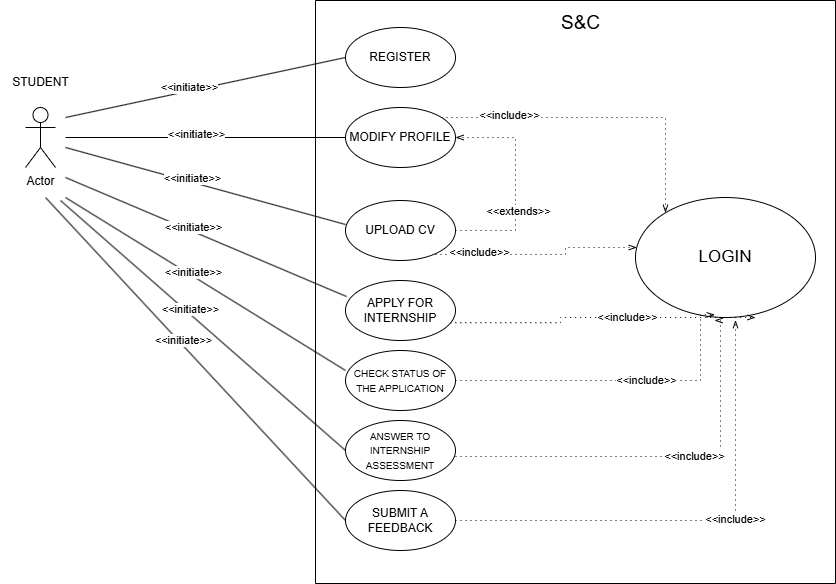
\includegraphics[scale=0.40]{images/ScenariosStateDiagram-UseCaseDiagrams_Student.drawio.png}
    \caption{Student use case diagram}
\end{figure}

\begin{figure}[ht!]
    \centering
    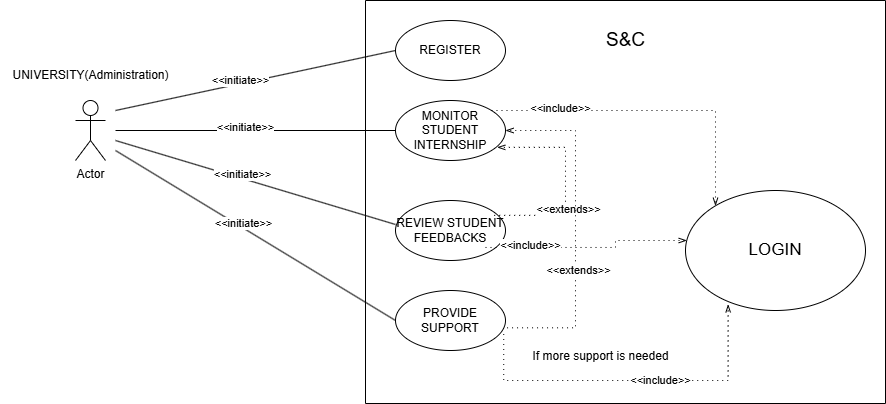
\includegraphics[scale=0.40]{images/ScenariosStateDiagram-UseCaseDiagram_Universities.drawio.png}
    \caption{University use case diagram}

\end{figure}

\begin{figure}[ht!]
    \centering
    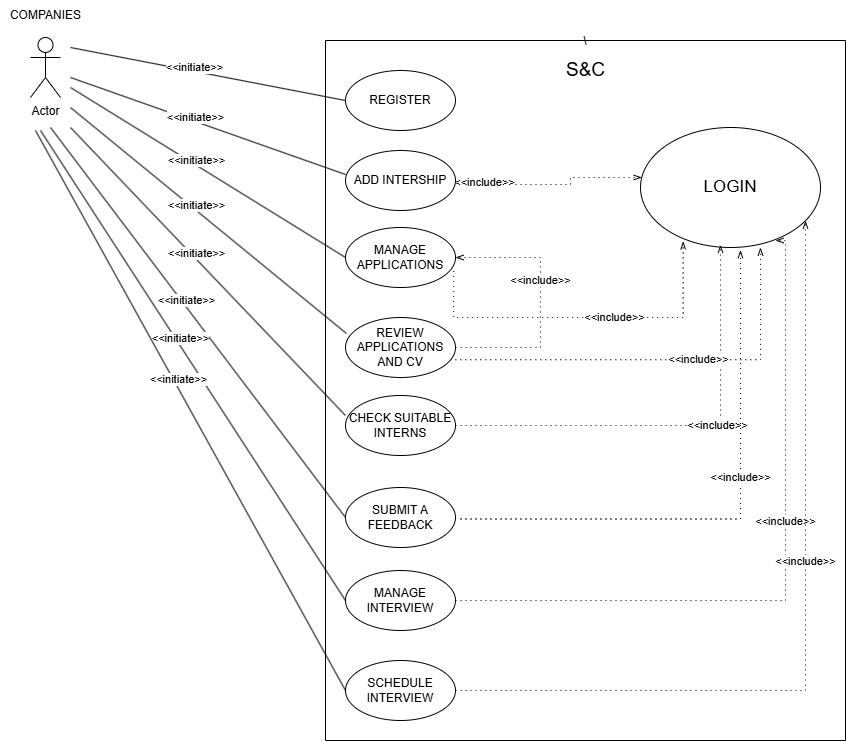
\includegraphics[scale=0.40]{images/ScenariosStateDiagram-UseCaseDiagram_Companies.drawio.png}
    \caption{Company use case diagram}

\end{figure}

\clearpage

\subsubsection{Use cases} 
\textbf{1) User registration use case}\\
\begin{table}[h!]
    \centering
    \begin{tabular}{lp{10cm}}
        \textbf{Actor} & User \\ \hline
        \textbf{Entry conditions} & The user is on the registration page of the S\&C platform and is ready to provide email and password. \\ \hline
        \textbf{Event Flow} & 
       1. The user enters email and password. \\
        & 2. S\&C platform validates the email and password. \\
        & 3a. If the email is already registered, the platform displays an error: "Email already registered, please enter a new email". \\
        & 3b. The user enters a new email. \\
        & 4. If the data is valid, the registration is successful. \\
        & 5. S\&C platform sends a confirmation email to the user via the Mail Server. \\
        & 6. The user receives the confirmation email. \\
        & 7a. she user clicks the confirmation link within 24 hours. \\
        & 7b. If not, the user can request to resend the confirmation email. \\
        \hline
        \textbf{Exit condition} & The user's email is confirmed, and the registration process is successfully completed. \\ \hline
        \textbf{Exceptions} & 
        3.1. The email is already registered, and the user must enter a new email. \\
        & 7.1. The user does not confirm the email within 24 hours and must request a new confirmation email. \\
    \end{tabular}
    \caption{User registration use case}
    \label{tab:user_registration}
\end{table}


\begin{center}
    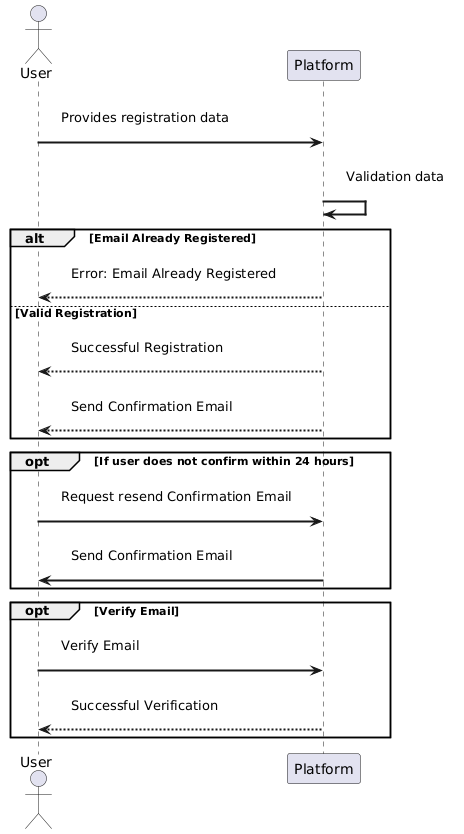
\includegraphics[scale = 0.5]{images/user_registration.png}
\end{center}
\newpage
\textbf{2) Student Login}\\

\begin{table}[h!]
    \centering
    \begin{tabular}{lp{10cm}}
        \textbf{Actor} & User \\ \hline
        \textbf{Entry conditions} & The user is on the login page of the S\&C platform, ready to enter credentials. \\ \hline
        \textbf{Event Flow} & 
        1. The user enters their email and password. \\
        & 2. The S\&C platform validates the credentials. \\
        & 3a. If the credentials are valid, the platform successfully logs in the user. \\
        & 3b. If the credentials are invalid, the platform returns an error: "Invalid email or password, please try again." \\
        \hline
        \textbf{Exit condition} & The user is logged into the platform if the credentials are valid. \\ \hline
        \textbf{Exceptions} & 
        3.1. Invalid email or password: the user must re-enter the correct credentials to log in. \\
    \end{tabular}
    \caption{User login use case}
    \label{tab:user_login}
\end{table}


\begin{center}
    \includegraphics[scale = 0.8]{images/Student_login.png}
\end{center}

\newpage
\textbf{3) Internship post creation use case}\\

\begin{table}[h!]
    \centering
    \begin{tabular}{lp{10cm}}
        \textbf{Actor} & Company \\ \hline
        \textbf{Entry conditions} & The company is on the S\&C platform, ready to create a new internship post. \\ \hline
        \textbf{Event Flow} & 
        1. The company fills out the internship information form. \\
        & 2. The S\&C platform validates the internship data. \\
        & 3a. If the data is valid, the platform creates the new internship post and confirms success to the company. \\
        & 3b. If the data is invalid, the platform returns an error: "Error in internship data, please correct the form." \\
        & 4. The company resubmits the corrected form, repeating the process until valid data is provided. \\
        & 5. The platform performs matching to find relevant students for the internship post. \\
        & 6. For each student that matches, the platform sends an internship post notification. \\
        \hline
        \textbf{Exit condition} & A new internship post is successfully created on the platform, and notifications are sent to relevant students. \\ \hline
        \textbf{Exceptions} & 
        3.1. Invalid internship data: The company must correct and resubmit the form until valid data is provided. \\
    \end{tabular}
    \caption{Internship post creation use case}
    \label{tab:internship_post_creation}
\end{table}



\begin{center}
    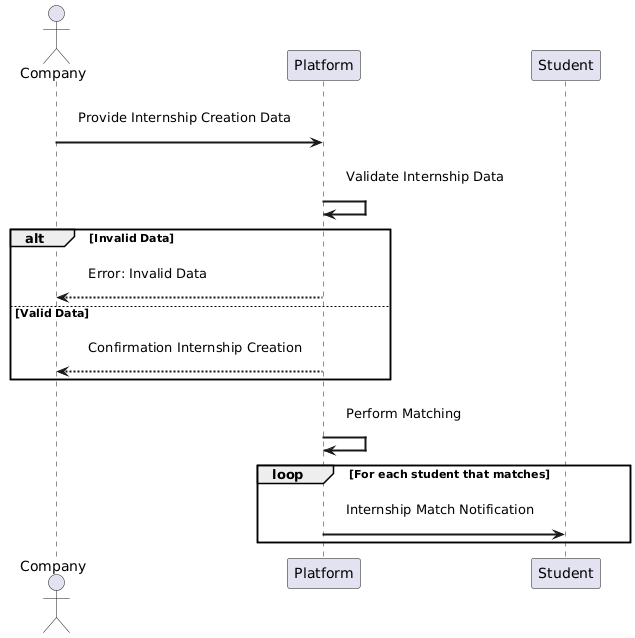
\includegraphics[scale = 0.8]{images/Internship_post_creation_use_case.png}
\end{center}

\newpage
\textbf{4) Personal data and CV upload use case}\\

\begin{table}[h!]
    \centering
    \begin{tabular}{lp{10cm}}
        \textbf{Actor} & Student \\ \hline
        \textbf{Entry conditions} & The student is on the S\&C platform, ready to submit personal data and optionally upload a CV. \\ \hline
        \textbf{Event Flow} & 
        1. The student submits their skills, interests, and other personal data. \\
        & 2a. If the personal data is invalid, the platform returns an error: "Error in personal data, please correct it." \\
        & 2b. If the personal data is valid, the platform confirms that the data was successfully uploaded. \\
        & 3. The student optionally uploads their CV. \\
        & 4a. If the CV is invalid, the platform returns an error: "Error in CV, please re-upload." \\
        & 4b. If the CV is valid, the platform confirms that the upload was successful. \\
        & 5. The platform performs matching based on the student data. \\
        & 6. For each matching company, the platform sends a notification about the student. \\
        \hline
        \textbf{Exit condition} & The student's personal data and, if applicable, CV are successfully uploaded and relevant companies are notified. \\ \hline
        \textbf{Exceptions} & 
        2.1. Invalid personal data: The student must correct and resubmit their personal data. \\
        & 4.1. Invalid CV: The student must re-upload their CV until it meets the platform's requirements. \\
    \end{tabular}
    \caption{Student personal data and CV upload use case}
    \label{tab:student_data_cv_upload}
\end{table}



\begin{center}
    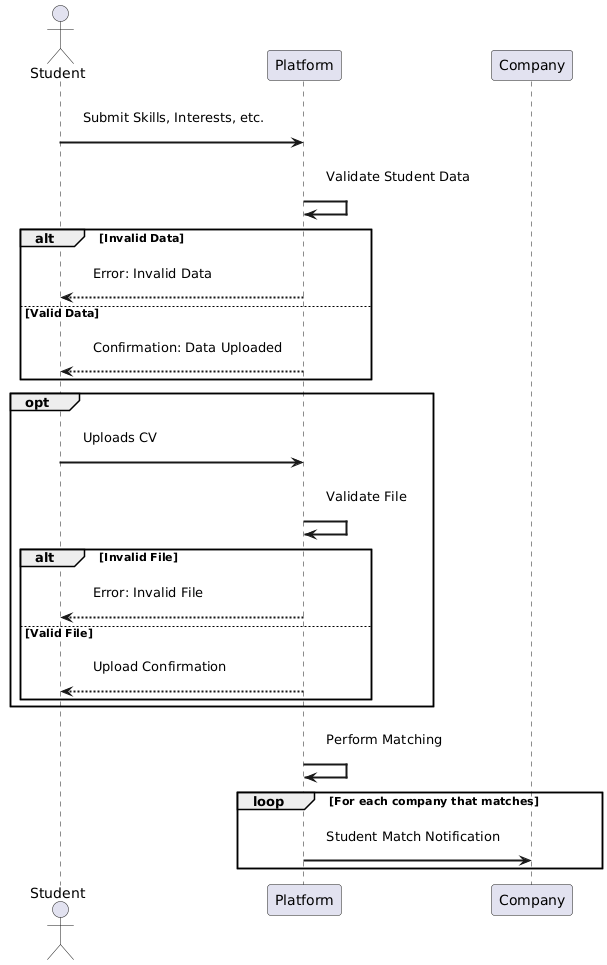
\includegraphics[scale = 0.8]{images/Personal_data_and_CV_upload.png}
\end{center}

\newpage
\textbf{5) Student application use case}\\

\begin{table}[h!]
    \centering
    \begin{tabular}{lp{10cm}}
        \textbf{Actor} & Student \\ \hline
        \textbf{Entry conditions} & The student is on the S\&C platform, ready to apply for an internship. \\ \hline
        \textbf{Event Flow} & 
        1. The student requests a list of internships. \\
        & 2. The platform provides the list of available internships. \\
        & 3. The student selects an internship from the list. \\
        & 4. The platform displays the details of the selected internship. \\
        & 5. The student submits their application data for the selected internship. \\
        & 6. The platform validates the application data. \\
        & 7a. If the data is valid, the platform confirms that the application submission was successful. \\
        & 7b. If the data is not valid, the platform returns an error message. \\
        & 8. If valid, the platform sends the application to the company. \\
        \hline
        \textbf{Exit condition} & The student's application for the internship is successfully submitted and sent to the company if the data is valid. \\ \hline
        \textbf{Exceptions} & 
        7.1. Invalid application data: The student must correct and resubmit their application data until it meets the platform's requirements. \\
    \end{tabular}
    \caption{Internship application use case}
    \label{tab:internship_application}
\end{table}


\begin{center}
    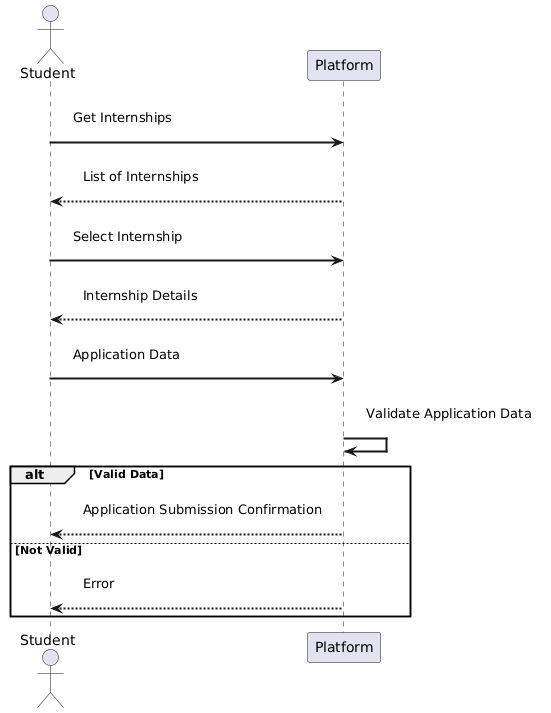
\includegraphics[scale = 0.8]{images/Student_application.png}
\end{center}

\newpage
\subsubsection{Summary of the Functional Requirements}
\begin{longtable}{|p{0.1\textwidth}|p{0.9\textwidth}|}
\hline
\textbf{R1} & The S\&C shall allow students to view a personalized dashboard displaying recommended internships, application statuses, and feedback. \\ 
\hline
\textbf{R2} & The S\&C shall allow students to create and edit profiles, upload CVs, and receive real-time validation. \\ 
\hline
\textbf{R3} & The S\&C shall allow students to access a search tool with filtering options for location, field of study, and required skills. \\ 
\hline
\textbf{R4} & The S\&C shall allow students to be guided through the application process with a step-by-step wizard, displaying deadlines and tracking progress. \\ 
\hline
\textbf{R5} & The S\&C shall allow companies to create, edit, and delete internship postings, including job roles and required skills. \\ 
\hline
\textbf{R6} & The S\&C shall allow companies to have a dashboard to review candidate applications, filter profiles, and schedule interviews. \\ 
\hline
\textbf{R7} & The S\&C shall allow companies to have a recommendation feed for candidates based on internship requirements. \\ 
\hline
\textbf{R8} & The S\&C shall allow universities to have an administrative dashboard to monitor internship progress and manage complaints. \\ 
\hline
\textbf{R9} & The S\&C shall allow universities to log, track, and update complaint statuses within a complaint management system. \\ 
\hline
\textbf{R10} & The S\&C shall allow integration with university databases via secure Restful APIs for verifying student enrollment and monitoring internship progress. \\ 
\hline
\textbf{R11} & The S\&C shall allow API integration with external career platforms and feedback tools for gathering insights on internship performance. \\ 
\hline
\textbf{R12} & The S\&C shall allow push notifications for web and mobile platforms, notifying users in real-time. \\ 
\hline
\textbf{R13} & The S\&C shall allow students to create and manage profiles, including personal details, education history, skills, and work experience. \\ 
\hline
\textbf{R14} & The S\&C shall allow companies to specify deadlines for internship postings, with automatic removal of expired listings. \\ 
\hline
\textbf{R15} & The S\&C shall allow the recommendation engine to improve over time based on feedback from student internships. \\ 
\hline
\textbf{R16} & The S\&C shall allow companies to manage interview schedules and log outcomes, including scores and feedback. \\ 
\hline
\textbf{R17} & The S\&C shall allow both students and companies to provide feedback post-internship, covering skills demonstrated and overall satisfaction. \\ 
\hline
\textbf{R18} & The S\&C shall allow universities to access a complaint management system for reviewing and resolving student-company issues. \\ 
\hline
\textbf{R19} & The S\&C shall allow a secure messaging system for direct communication between students and companies while preserving user privacy. \\ 
\hline
\textbf{R20} & The S\&C shall allow companies access to a comprehensive analytics dashboard to analyze candidate engagement, track application trends, and optimize postings. \\ 
\hline
\textbf{R21} & The S\&C shall allow students to set career goals and objectives, with tailored internship suggestions based on these goals. \\ 
\hline
\textbf{R22} & The S\&C shall allow users to select their preferred language from platform settings to enhance accessibility. \\ 
\hline
\textbf{R23} & The S\&C shall allow companies to access a "Similar Candidates" feature to view potential matches based on applicant profiles. \\ 
\hline
\textbf{R24} & The S\&C shall allow a feedback mechanism for students to receive suggestions for improving profiles, including skill recommendations based on industry trends. \\ 
\hline
\textbf{R25} & The S\&C shall allow students and companies to rate each other post-internship, contributing to a reputation score visible to other users. \\ 
\hline
\textbf{R26} & The S\&C shall allow a periodic internship recommendation email digest for students who opt-in, summarizing new or high-match opportunities. \\ 
\hline
\textbf{R27} & The S\&C shall allow students to track essential pre- and post-internship tasks and documents with a "Checklist" tool. \\ 
\hline
\textbf{R28} & The S\&C shall allow companies access to templates and guidelines for internship descriptions to standardize postings and attract suitable candidates. \\ 
\hline
\textbf{R29} & The S\&C shall allow students to recommend other students for internships, fostering peer networking through a referral feature. \\ 
\hline
\textbf{R30} & The S\&C shall allow integration of two-factor authentication for enhanced security of student and company accounts. \\ 
\hline
\textbf{R31} & The S\&C shall allow encryption of all sensitive user data, ensuring compliance with data protection regulations. \\ 
\hline
\textbf{R32} & The S\&C shall allow a help center with FAQs and live chat support for real-time assistance for students, companies, and university administrators. \\ 
\hline
\textbf{R33} & The S\&C shall allow automated reminders for companies about pending feedback or assessments for completed internships. \\ 
\hline
\textbf{R34} & The S\&C shall allow students to mark internships as "favorites" or for easy reference during application. \\ 
\hline
\textbf{R35} & The S\&C shall allow companies to post exclusive internships targeted to students from specific universities or programs. \\ 
\hline
\textbf{R36} & The S\&C shall allow students access to an analytics page showing internship trends, including popular industries, roles, and demanded skills. \\ 
\hline
\textbf{R37} & The S\&C shall allow students and companies access to a document management tool for secure uploading, storing, and sharing of internship-related documents. \\ 
\hline
\textbf{R38} & The S\&C shall allow companies to set internship visibility criteria, such as grade level, skill sets, and field of study. \\ 
\hline
\textbf{R39} & The S\&C shall allow universities access to an analytics dashboard to track student engagement, successful matches, and completion rates. \\ 
\hline
\textbf{R40} & The S\&C shall allow a reporting feature for users to report inappropriate or irrelevant internship environment, ensuring a safe and professional place. \\ 
\hline
\textbf{R41} & The S\&C shall allow personalized reminders for students, notifying them of application deadlines, interview dates, and required documents. \\ 
\hline
\textbf{R42} & The S\&C shall allow students to set privacy levels on their profiles, determining what details are public to companies or universities. \\  
\hline
\textbf{R43} & The S\&C shall allow integration with calendars for synchronizing dates like interview or deadline dates. \\ 
\hline
\textbf{R44} & The S\&C shall allow a section with the best internship sorted by feedbacks. \\ 
\hline
\textbf{R45} & The S\&C shall allow students to view average application review times by companies via an "Application Insights" feature. \\ 
\hline
\textbf{R46} & The S\&C shall allow an assessment tool for students to understand and showcase non-technical strengths. \\ 
\hline
\textbf{R47} & The S\&C shall allow tracking of job market trends, notifying students of growing fields to help adapt skills according to their matching features. \\ 
\hline
\textbf{R48} & The S\&C shall allow endorsements from companies and universities, adding credibility to student profiles for specific skills. \\ 
\hline
\textbf{R49} & The S\&C shall allow a real-time "Internship Analytics" page for universities, summarizing internship data like completion rates. \\ 
\hline
\textbf{R50} & The S\&C shall allow companies a Candidate Comparison tool for side-by-side candidate evaluation. \\ 
\hline
\textbf{R51} & The S\&C shall allow real-time tracking of application statuses, showing students the progress of applications at each stage. \\ 
\hline
\textbf{R52} & The S\&C shall allow a recommendation ranking feature to help students prioritize opportunities based on match percentage and goals. \\ 
\hline
\textbf{R53} & The S\&C shall allow an internship recommendation score based on student profiles, skills. \\ 
\hline
\textbf{R54} & The S\&C shall allow companies to provide additional criteria\\
\hline
\end{longtable}
\newpage
\subsubsection{Mapping on Goals}
In the following table it is shown how the different goals map on the requirements and domain assumptions described in the previous chapters. Furthermore, the mapping is made in order to make this formula hold 
\begin{equation}
R \land D \models G
\end{equation}
\begin{longtable}{| p{0.3\textwidth} | p{0.4\textwidth} | p{0.4\textwidth} |}
\hline
\textbf{Goal} & \textbf{Domain Assumptions (DA)} & \textbf{Requirements (R)} \\ 
\hline
G1: Enable students to search for internships that match their skills and career goals. & DA1: Students need internships to gain practical experience. \newline DA3: Students have varied skills and interests. \newline DA5: Students need to provide a valid email address. \newline DA8: Both students and companies need to have a connection and a device to connect to the platform. & R1: Display a personalized dashboard with recommended internships, application statuses, and feedback. \newline R2: Allow students to create/edit profiles, upload CVs, and validate them in real-time. \newline R3: Provide a search tool with filtering options. \newline R4: Guide students through applications with a step-by-step wizard. \newline R21: Enable students to set career goals and receive tailored internship suggestions. \newline R52: Provide a recommendation ranking feature to help students prioritize opportunities. \\ \hline

G2: Provide companies with tools to advertise internships and attract suitable candidates. & DA2: Companies need interns for various projects. \newline DA4: Companies have specific internship requirements. \newline DA6: Companies need to provide a valid email. \newline DA8: Both parties need connectivity to the platform. & R5: Enable companies to manage internship postings with job roles and skill requirements. \newline R6: Provide a dashboard for companies to review applications, filter profiles, and schedule interviews. \newline R14: Allow companies to specify deadlines for postings, with expired listings automatically removed. \newline R20: Give companies access to analytics for candidate engagement and application trends. \newline R28: Provide templates and guidelines to standardize internship descriptions. \newline R38: Allow companies to set visibility criteria based on grade level, skills, and field of study. \\ \hline

G3: Offer recommendation mechanisms for students to match with relevant internships. & DA3: Students have varied skills and interests. \newline DA4: Companies have specific internship requirements. & R7: Provide companies with a recommendation feed based on internship requirements. \newline R15: Improve the recommendation engine over time based on feedback from completed internships. \newline R21: Allow students to set career goals for more tailored suggestions. \newline R52: Enable students to prioritize opportunities with a ranking feature. \newline R53: Generate internship recommendation scores based on student profiles and past performance. \\ \hline

G4: Offer recommendation mechanisms for companies to find potential candidates. & DA2: Companies need interns for various projects. \newline DA4: Companies have specific internship requirements. & R6: Provide companies with a dashboard to review applications and filter profiles. \newline R7: Offer companies a recommendation feed for candidates. \newline R23: Show companies "Similar Candidates" based on profiles. \newline R50: Include a "Candidate Comparison" tool for companies to evaluate applicants side-by-side. \\ \hline

G5: Facilitate the selection process through an interview management system. & DA2: Companies need interns for various projects. \newline DA4: Companies have specific internship requirements. & R5: Enable companies to create and manage internship postings. \newline R6: Provide companies a dashboard to review and manage candidate applications. \newline R16: Support interview scheduling and logging, including scores and feedback. \newline R20: Include a comprehensive analytics dashboard for tracking trends. \newline R68: Allow additional selection criteria like language requirements. \\ \hline

G6: Supports the candidate's evaluation. & DA4: Companies have specific internship requirements. \newline DA9: Universities are interested in monitoring internship quality. & R16: Support interview scheduling and recording outcomes. \newline R17: Enable feedback mechanisms post-internship for skills and satisfaction. \newline R50: Provide a comparison tool for side-by-side candidate evaluation. \\ \hline

G7: Gather feedback from students and companies to continuously improve the matchmaking process. & DA3: Students have varied skills and interests. \newline DA4: Companies have specific internship requirements. \newline DA9: Universities are interested in monitoring internship quality. & R15: Continuously improve the recommendation engine with feedback. \newline R17: Facilitate feedback post-internship. \newline R24: Offer profile improvement suggestions, including skill recommendations. \newline R33: Send automated reminders for companies to provide feedback. \newline R44: Include a "Success Stories" section showcasing successful internships. \\ \hline

G8: Enable universities to monitor internship progress and manage potential issues. & DA9: Universities are interested in monitoring internship quality. \newline DA7: Universities need to have a valid email. & R8: Allow universities to access an administrative dashboard for monitoring. \newline R9: Provide a complaint management system for universities. \newline R10: Integrate with university databases for student verification and internship progress monitoring. \newline R39: Enable universities to access analytics on engagement and completion rates. \newline R49: Show universities a real-time "Internship Analytics" page summarizing internship data. \\ \hline
\end{longtable}



\begin{itemize}
    \item \textbf{Student Profile Management}: 
        \begin{itemize}
            \item Students can create and manage profiles, including personal details, education history, skills, and work experience.
            \item The profile interface will support dynamic updates, and validation of critical fields to ensure profile completeness.
            \item Uploaded CVs must be in PDF or DOCX format, and the system must validate that the upload meets the required format.
            \item Profiles must support a review system where students can preview how their information will appear to potential employers.
        \end{itemize}
    \item \textbf{Internship Listings}: 
        \begin{itemize}
            \item Companies can create, update, and delete internship listings with detailed descriptions, requirements, and benefits.
            \item Listings must include filters for location, skills, and compensation, allowing students to search effectively.
            \item The system must allow companies to specify internship deadlines, and automatically remove expired listings.
            \item A dynamic feedback mechanism will notify companies about the completeness and attractiveness of their internship postings, suggesting improvements if needed.
        \end{itemize}
    \item \textbf{Recommendation System}: 
        \begin{itemize}
            \item The recommendation engine must take into account factors such as the student’s skills, location preferences, previous internships, and company requirements.
            \item The engine will learn and improve over time using feedback data from previous internships, adjusting future recommendations based on the outcomes and feedback provided by both students and companies.
        \end{itemize}
    \item \textbf{Selection and Interview Process}: 
        \begin{itemize}
            \item Companies can select candidates for interviews and manage interview schedules directly through the platform.
            \item Structured questionnaires will be provided by companies for student applicants to complete prior to interviews, with results stored in the system for company review.
            \item Companies will be able to log interview outcomes, including scores and qualitative feedback, directly into the system to aid decision-making.
        \end{itemize}
    \item \textbf{Feedback Collection}: 
        \begin{itemize}
            \item After each internship, both students and companies must provide structured feedback on the experience.
            \item The feedback must cover multiple dimensions, including skills demonstrated, professionalism, and overall satisfaction.
            \item The system will anonymize feedback to comply with GDPR regulations, ensuring privacy for both parties involved.
            \item The feedback will be used as a data source for improving the recommendation system and internship matching algorithm.
        \end{itemize}
    \item \textbf{Complaint Handling}: 
        \begin{itemize}
            \item Universities must have access to a complaint management system, allowing them to view and manage complaints filed by either students or companies.
            \item Complaints must be classified by type (e.g., harassment, contract breach) and tracked through a resolution workflow.
            \item Complaints can be escalated for review by a university administrator, who will have access to the full history of the issue.
            \item The system will automatically notify all relevant parties (students, companies, administrators) of complaint status updates.
        \end{itemize}
\end{itemize}

\subsection{Performance Requirements}

\subsubsection{Number of Users}
The platform will be used by multiple parties, including students, companies, and universities. Based on market research, which includes a comparison with existing similar platforms such as the CareerService platform for Politecnico di Milano (Polimi) and other internship-matching services across Europe, we estimate that S\&C will attract approximately 20,000 students and 2,500 companies from various universities and industries. Additionally, around 50 universities will be actively using the platform to monitor internships. This gives us an estimated total user base of 22,550 users.\\ \\
Considering a worst-case scenario where 40\% of the users are active simultaneously, the system must support up to 9,020 concurrent users. The platform must ensure smooth operation, even during peak usage times.

\subsubsection{Data Storage}
The platform needs to store various types of data related to students, companies, internships, and the matchmaking process. Below are the estimated storage requirements for the first year of operation:

\begin{itemize}
    \item \textbf{Student data (profile)}: Each student will have a profile containing personal information such as name, contact details, and skillset. This profile data is estimated to require around 10 KB per student. Considering 20,000 students:
    \[
    20,000 \times 10 \, \text{KB} = 195.3 \, \text{MB}
    \]
    
    \item \textbf{Student data (PDF CVs)}: In addition to the basic profile information, each student is expected to upload their CV in PDF format. The average size of a CV in PDF format is estimated to be around 300 KB. Thus, for 20,000 students:
    \[
    20,000 \times 300 \, \text{KB} = 5.72 \, \text{GB}
    \]
    
    \item \textbf{Company data}: Each company will have a profile including company information, project descriptions, and internship offerings. Assuming 15 KB of storage per company profile and considering 2,500 companies:
    \[
    2,500 \times 15 \, \text{KB} = 36.6 \, \text{MB}
    \]
    
    \item \textbf{Internship postings}: Each internship posting will include information about the project, tasks, technologies, and terms (e.g., paid/unpaid). Assuming each posting requires 10 KB and that each company posts five internships a year:
    \[
    2,500 \times 5 \times 10 \, \text{KB} = 122.1 \, \text{MB}
    \]
    
    \item \textbf{Student feedback and internship outcomes}: Feedback data provided by students and companies will be stored for analysis. Assuming 5 KB per feedback submission and expecting each internship to receive three feedback entries, for 10,000 matched internships in the first year:
    \[
    10,000 \times 3 \times 5 \, \text{KB} = 146.5 \, \text{MB}
    \]
    
    \item \textbf{Interview and selection data}: Information about interviews, questionnaires, and selection processes will also be stored. Assuming 8 KB per interview record and that each company interviews an average of five candidates per internship:
    \[
    10,000 \times 5 \times 8 \, \text{KB} = 390.6 \, \text{MB}
    \]
\end{itemize}

Summing all storage requirements for the first year:
\[
195.3 \, \text{MB} + 5.72 \, \text{GB} + 36.6 \, \text{MB} + 122.1 \, \text{MB} + 146.5 \, \text{MB} + 390.6 \, \text{MB} = 6.6 \, \text{GB}
\]\\
Thus, a storage allocation of \textbf{10 GB} will be sufficient to accommodate the platform's data storage needs for a year, including room for growth and additional data generated by the system.


\subsubsection{Time Response}
Although there are no strict time requirements for the S\&C platform, it is important to maintain a responsive user experience. Reasonable average response times for key interactions could be as follows:
\begin{itemize}
    \item Basic search queries and browsing operations should ideally be processed within \textbf{2 seconds}, to ensure a smooth navigation experience.
    \item More complex operations, such as generating personalized internship recommendations, should aim to complete within \textbf{5 seconds}, balancing the computational effort required with acceptable wait times for the user.
\end{itemize}

\subsection{Design Constraints}

\subsubsection{Standards Compliance}

The platform must adhere to EU's GDPR regulations to ensure secure data storage and transmission, particularly when handling sensitive student and company data. All data interactions must comply with GDPR provisions regarding data ownership, user consent, and the right to access and delete data.

Additionally, the platform must comply with industry security standards to ensure the system is secure against potential threats.

\subsubsection{Hardware Limitations}

There are no specific hardware limitations imposed on end-users.

\subsection{Software System Attributes}

\subsubsection{Reliability}
The S\&C platform must be reliable to ensure continuous operation, even in the presence of faults. The system should be designed to be fault-tolerant to prevent the propagation of errors and ensure uninterrupted usability. Mechanisms such as automated failover and data redundancy should be in place to mitigate the risk of downtime due to unexpected failures.

\subsubsection{Availability}
The platform must be available as much as possible, with a minimum uptime of 99.999\%. Scheduled maintenance breaks should be minimized and, when necessary, performed during low-traffic periods (e.g., nighttime) to avoid disrupting critical usage, particularly around high-demand periods such as internship application deadlines.

\subsubsection{Security}
Security is critical for the S\&C platform, as it handles sensitive student and company data. The system must implement strong authentication and authorization mechanisms. Authentication should ensure that users are properly identified before accessing the platform, while authorization should ensure that users can only perform actions they are permitted to.

\subsubsection{Maintainability}
The platform should be designed with scalability and modularity in mind to facilitate the easy addition of new features or modifications with minimal effort. The use of reusable code components and modular architecture will aid in making future updates efficient. Regular maintenance operations should be scheduled during times of low user activity, such as nighttime, to minimize disruptions to users.

\subsubsection{Portability}
The S\&C platform must be accessible from a wide range of web browsers, ensuring compatibility across all major platforms (e.g., Chrome, Firefox, Safari, and Edge). On the client side, the platform should support responsive design, making it accessible on both desktop and mobile devices. No specific portability requirements are imposed on the server side, provided the platform can run on common server configurations.


\newpage
